\documentclass{article}
\usepackage[T2A]{fontenc}
\usepackage[utf8]{inputenc}
\usepackage[russian]{babel}
\usepackage{amssymb,amsmath,amsthm}
\usepackage{systeme,mathtools}
\usepackage{lipsum}
\usepackage{relsize}
\newcommand\md{\ }
\usepackage[normalem]{ulem}
\usepackage{pdfpages}

\begin{document}
\selectlanguage{russian}

\includepdf[pages=-]{Ok.pdf}
\section{Задание}

1.Необходимо реализовать простейший класс Shape (Фигура) на языке программирования Java. Добавить метод toString(). Создать класс-тестер для вывода информации об объекте.

2. Реализуйте простейший класс «Мяч»

3. Реализуйте простейший класс «Книга»

4. Разработайте и реализуйте класс Dog (Собака), поля класса описывают кличку и возраст собаки. Необходимо выполнить следующие действия: определить конструктор собаки, чтобы принять и инициализировать данные экземпляра., включить стандартные методы (аксессоры) для получения и установки для имени и возраста, включить метод для перевода возраста собаки в "человеческий " возраст (возраст семь раз собаки), включите метод ToString, который возвращает описание экземпляра собаки в виде строки. Создание класса тестера под названием ПитомникСобак, реализует массив собак и основной метод этого класса позволяет добавить в него несколько объектов собаки.

\section{Ход работы}

В ходе выполнения работы были получены следующие исходные коды:

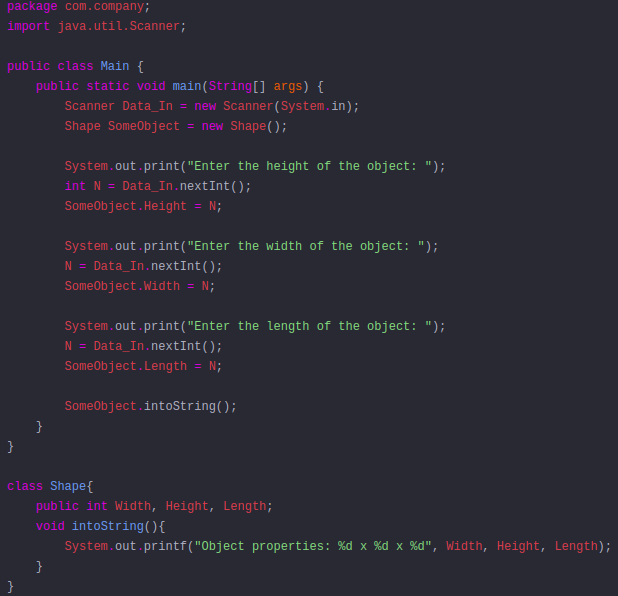
\includegraphics[width=0.7\linewidth]{view1.png}

\caption{Рисунок 1. Фрагмент кода для реализации задания с классом Shape.}

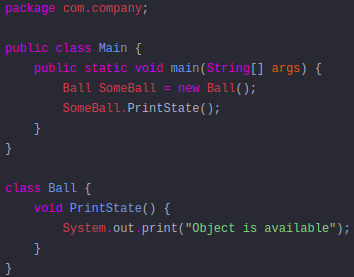
\includegraphics[width=0.9\linewidth]{view2.png}

\caption{Рисунок 2. Фрагмент кода для реализации задания с классом Ball (Мяч).}

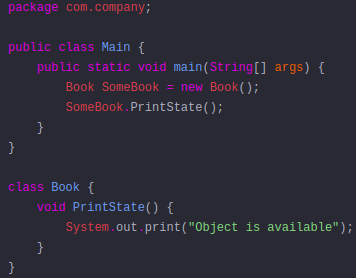
\includegraphics[width=0.9\linewidth]{view3.png}

\caption{Рисунок 3. Фрагмент кода для реализации задания с классрм Book (Книга).}

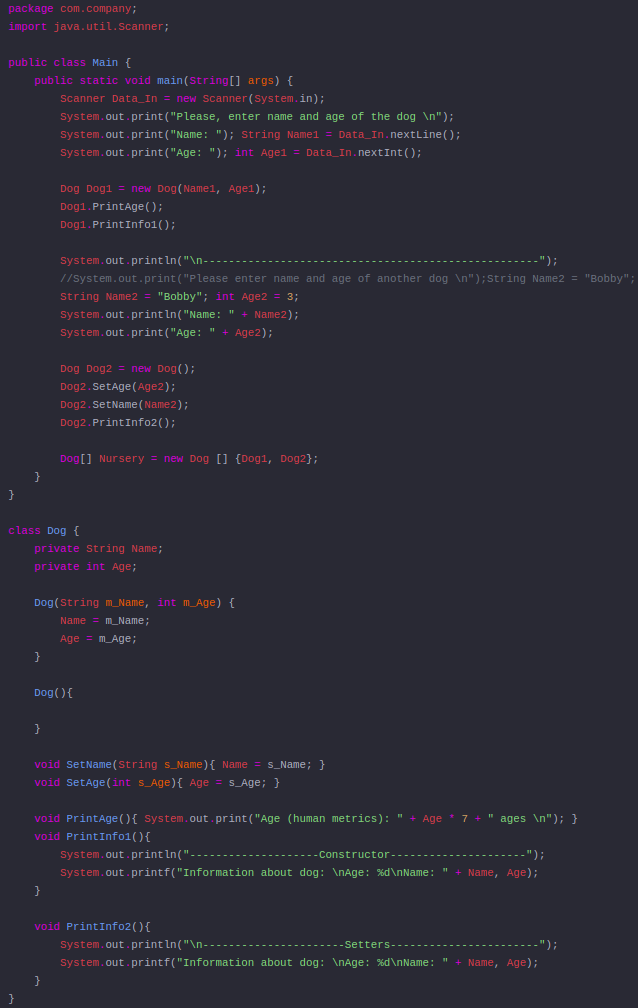
\includegraphics[width=0.94\linewidth]{view4.png}

\caption{Рисунок 4. Фрагмент кода для реализации задания с классом Dog (Собака).}

\section{Вывод}
В ходе выполнения практического занятия номер 2 я научилась реализовывать протсейшие классы на языке программирования Java.

\end{document}
